\chapter*{L’île de Pâques\markboth{L’île de Pâques}{}}
\section*{8 mars 2015}
Petite entorse au règlement du voyage, je suis parti 3 jours sur l'île de Pâques sans le vélo. Il est resté à Santiago chez Nelson, un chilien qui m'a hébergé en Couchsurfing.

 Camping au bord de l'océan dans la petite ville d'Hanga Roa, la seule de l'île.
\begin{center} 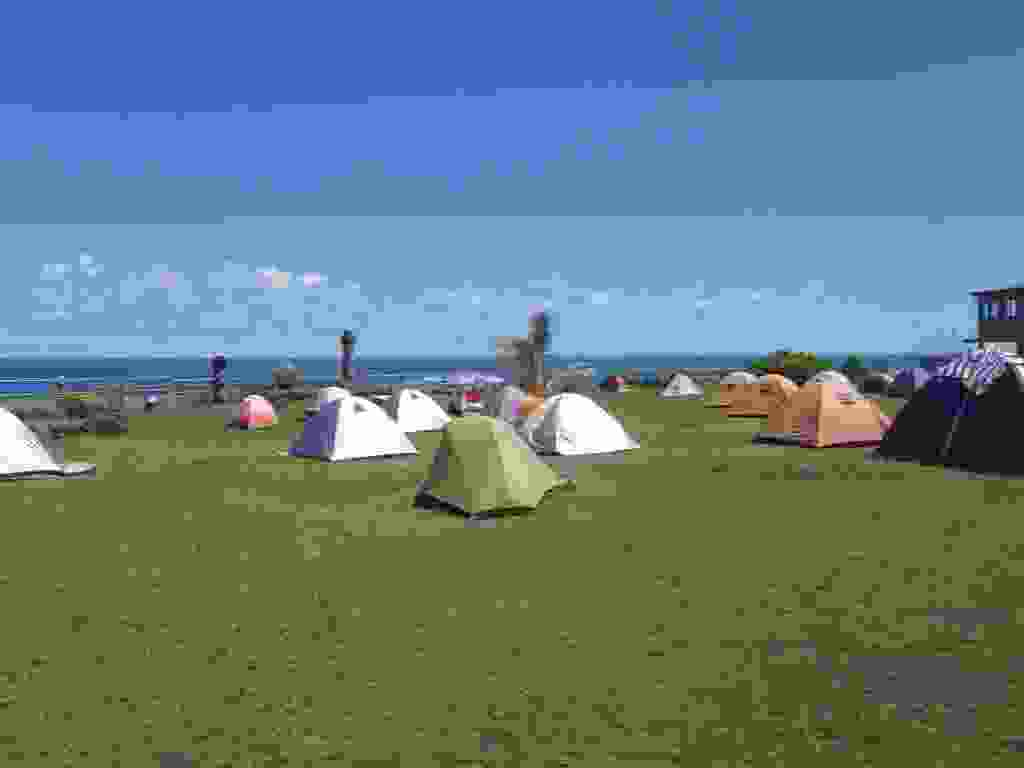
\includegraphics[width=\mywidth]{../wp-content/uploads/2015/03/P3012436-1024x768.jpg} \end{center}
\vspace{-\topsep}

\pagebreak
Petite balade au bord de l'eau et les premiers Moais sont là.
\begin{center} 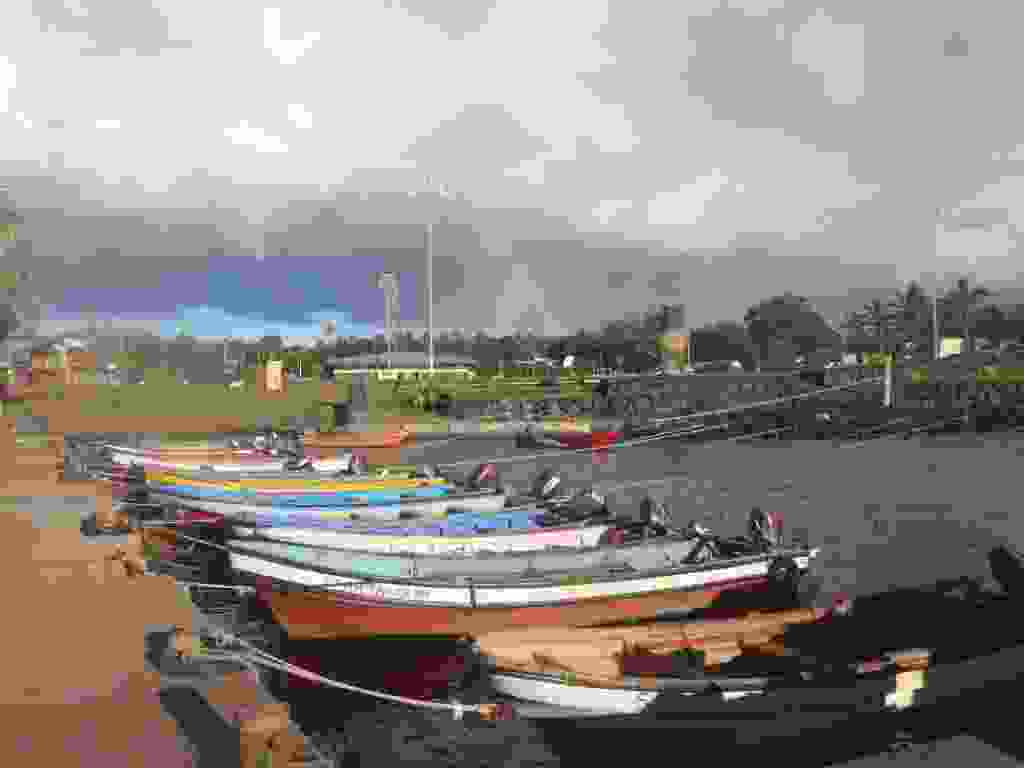
\includegraphics[width=\mywidth]{../wp-content/uploads/2015/03/P3032529-1024x768.jpg} \end{center}
\begin{center} 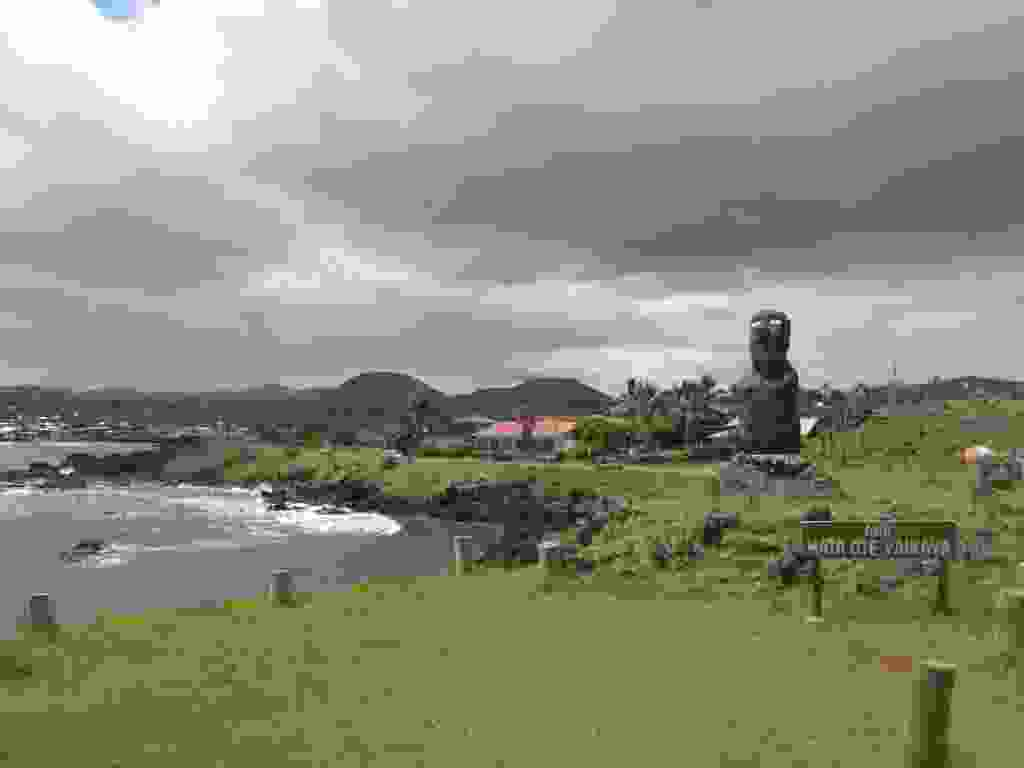
\includegraphics[width=\mywidth]{../wp-content/uploads/2015/03/P3012439-1024x768.jpg} \end{center}
\vspace{-\topsep}
\vspace{-3.25mm}

\pagebreak
~
\begin{center} 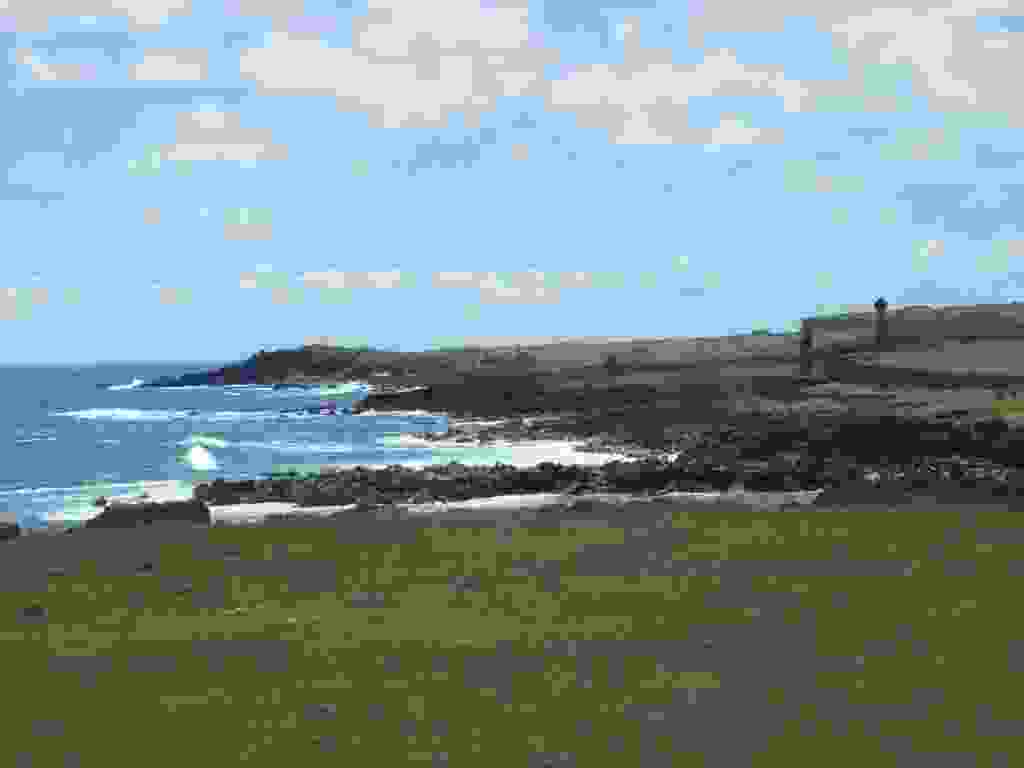
\includegraphics[width=\mywidth]{../wp-content/uploads/2015/03/P3012444-1024x768.jpg} \end{center}
\begin{center} 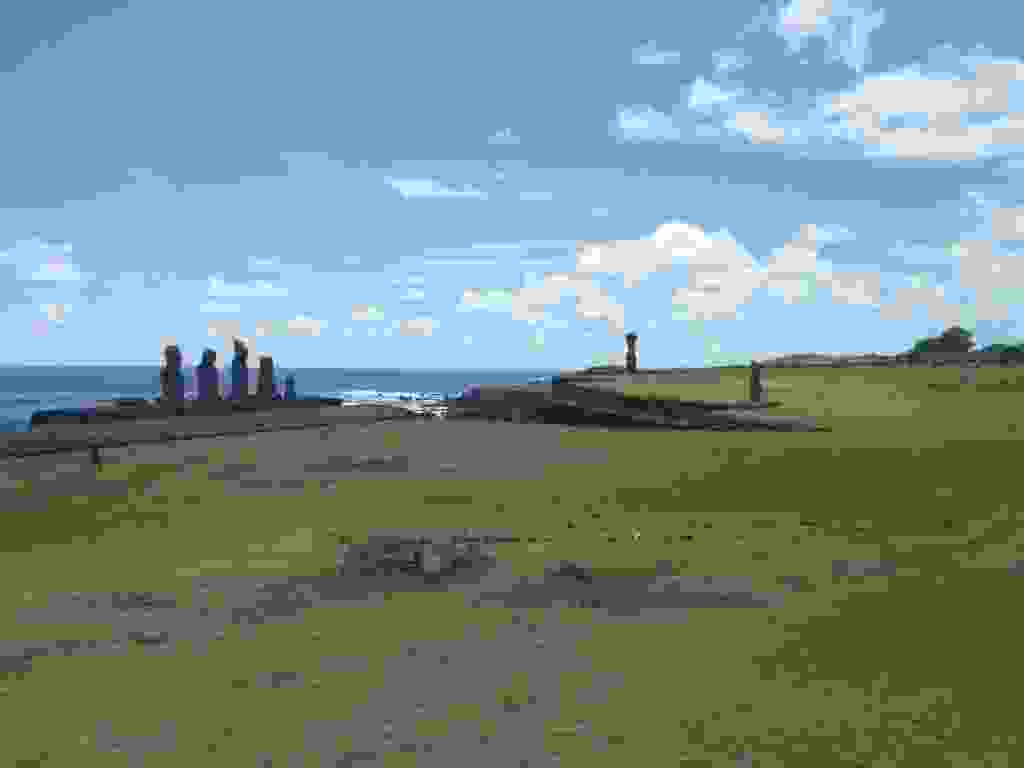
\includegraphics[width=\mywidth]{../wp-content/uploads/2015/03/P3012445-1024x768.jpg} \end{center}
\vspace{-\topsep}
\vspace{-3.25mm}

\begin{center} 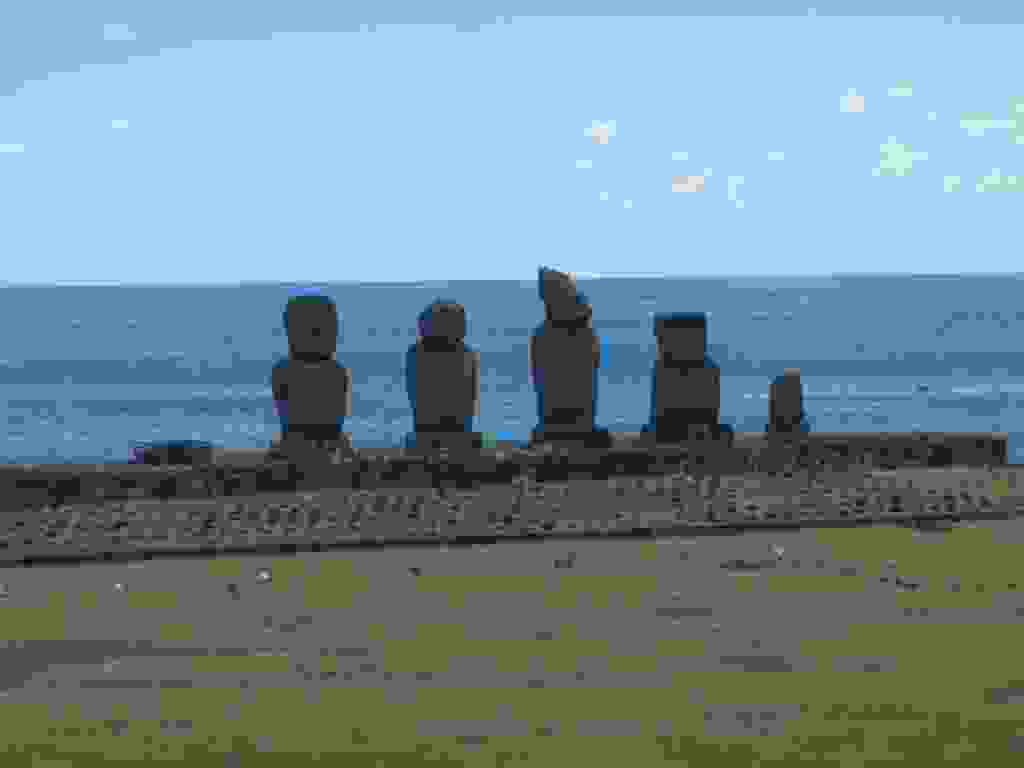
\includegraphics[width=\mywidth]{../wp-content/uploads/2015/03/P3012446-1024x768.jpg} \end{center}
\begin{center} 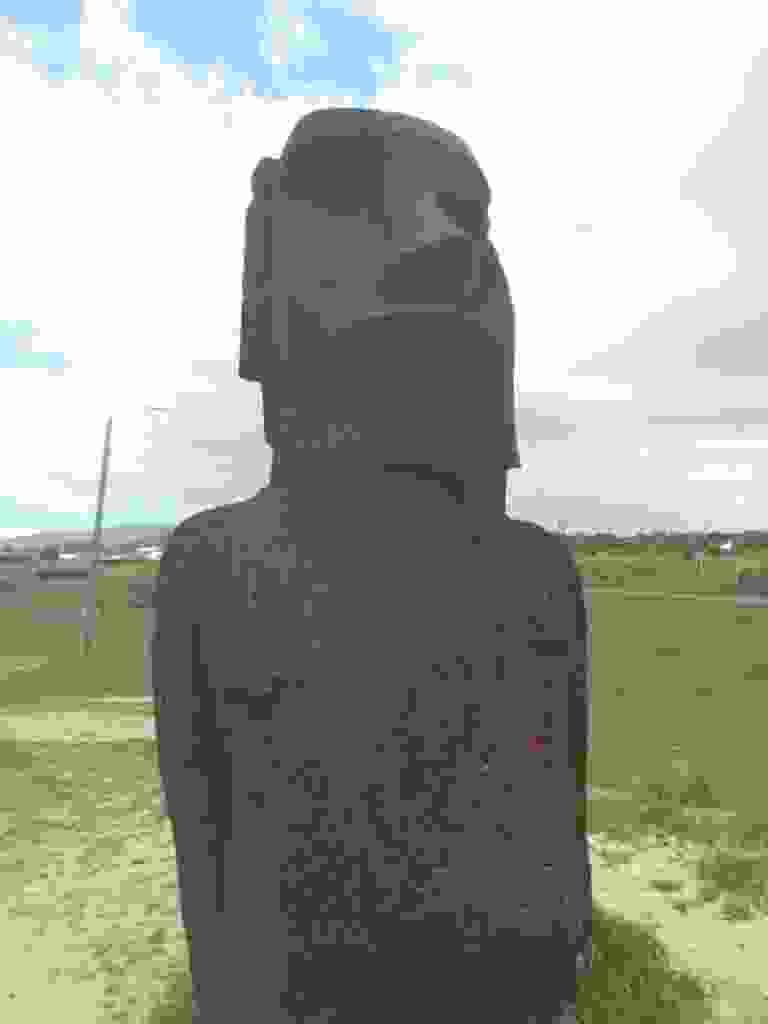
\includegraphics[height=\mywidth]{../wp-content/uploads/2015/03/P3012443-768x1024.jpg} \end{center}
\begin{center} 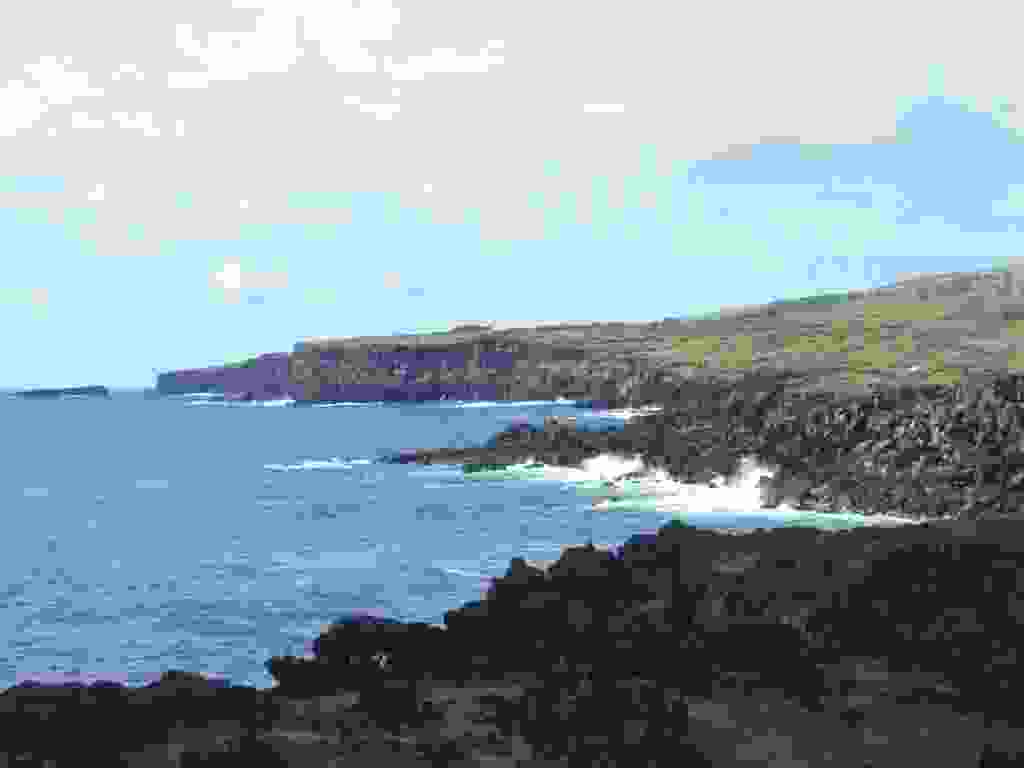
\includegraphics[width=\mywidth]{../wp-content/uploads/2015/03/P3022469-1024x768.jpg} \end{center}

 Le lendemain, j'ai loué une voiture avec 2 autres voyageurs rencontrés au camping.

 Départ à 7h pour aller voir le lever du soleil sur les 15 Moais d'Ahu Tongakiri, c'est le site où il y en a le plus debouts.
\begin{center} 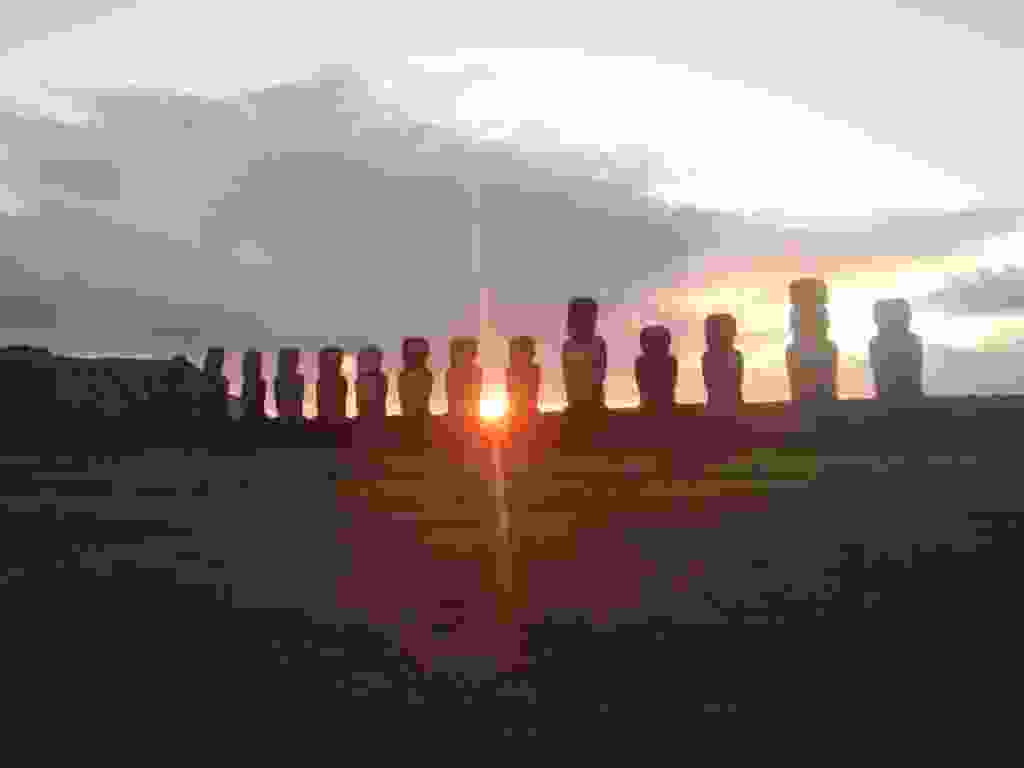
\includegraphics[width=\mywidth]{../wp-content/uploads/2015/03/P3022493-1024x768.jpg} \end{center}
\begin{center} 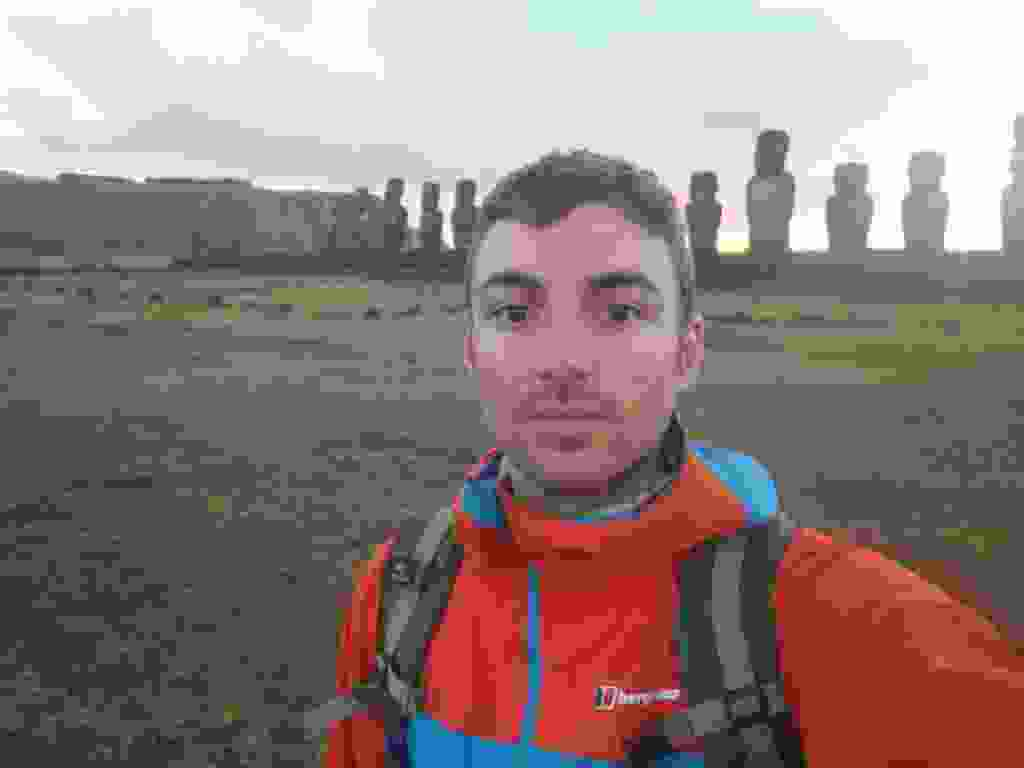
\includegraphics[width=\mywidth]{../wp-content/uploads/2015/03/P3022492-1024x768.jpg} \end{center}
\begin{center} 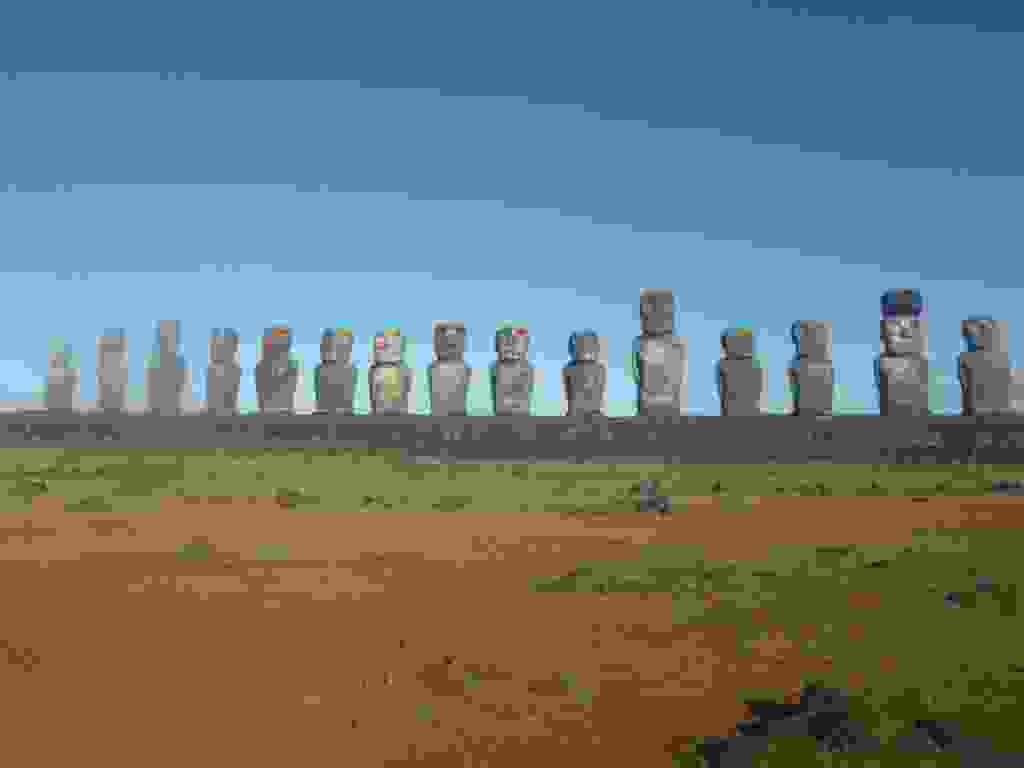
\includegraphics[width=\mywidth]{../wp-content/uploads/2015/03/P3032527-1024x768.jpg} \end{center}
\begin{center} 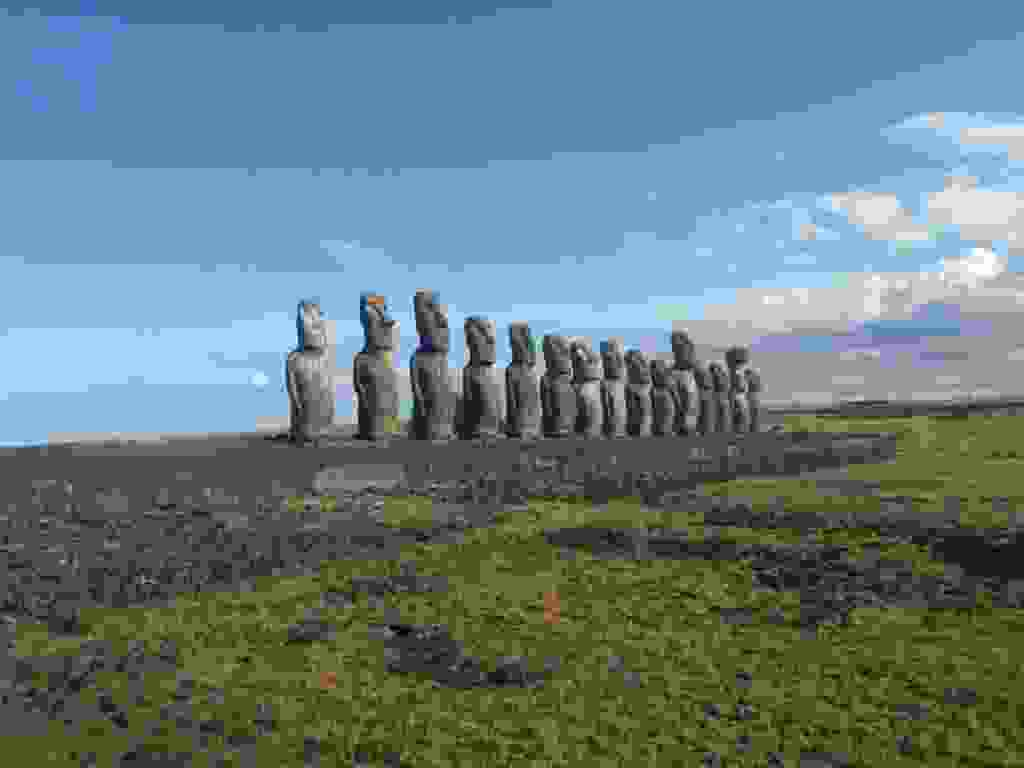
\includegraphics[width=\mywidth]{../wp-content/uploads/2015/03/P3032525-1024x768.jpg} \end{center}

Visite du site de Rano Raraku, là où les Moais ont été extraits de la roche, il en reste des dizaines inachevés ou en cours de déplacement.
\begin{center} 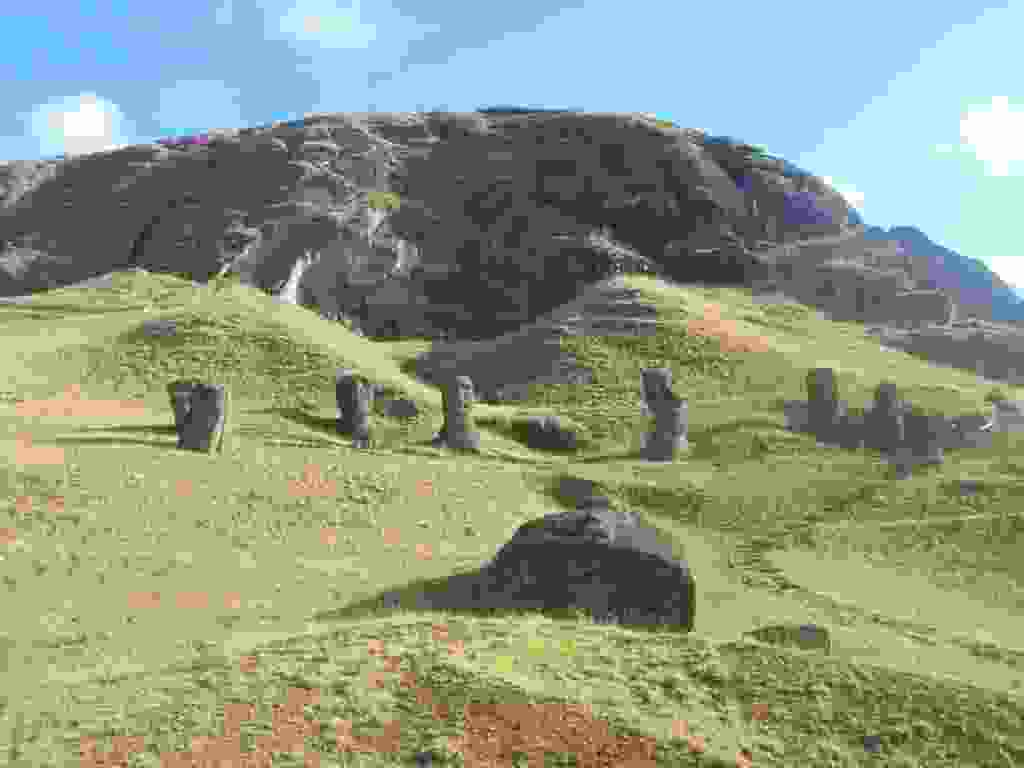
\includegraphics[width=\mywidth]{../wp-content/uploads/2015/03/P3022504-1024x768.jpg} \end{center}
\vspace{-\topsep}
\pagebreak
~\\
\begin{center} 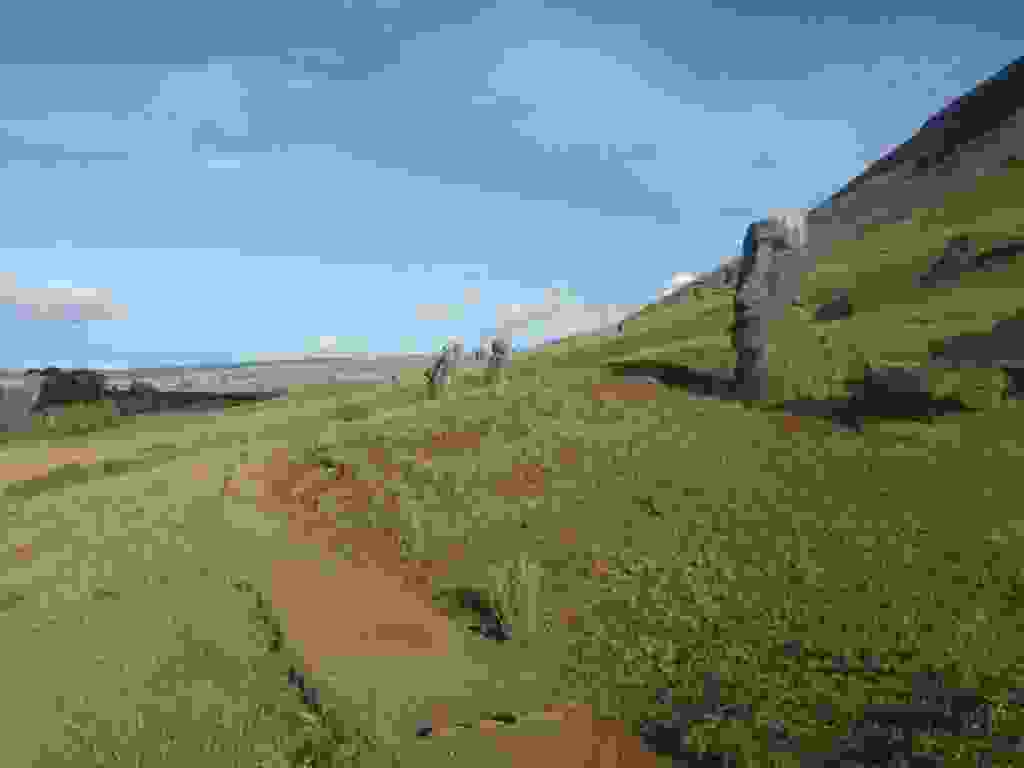
\includegraphics[width=\mywidth]{../wp-content/uploads/2015/03/P3022505-1024x768.jpg} \end{center}

 Nous sommes montés au volcan Maunga Terevaka, point culminant de l'île à 511m.
\begin{center} 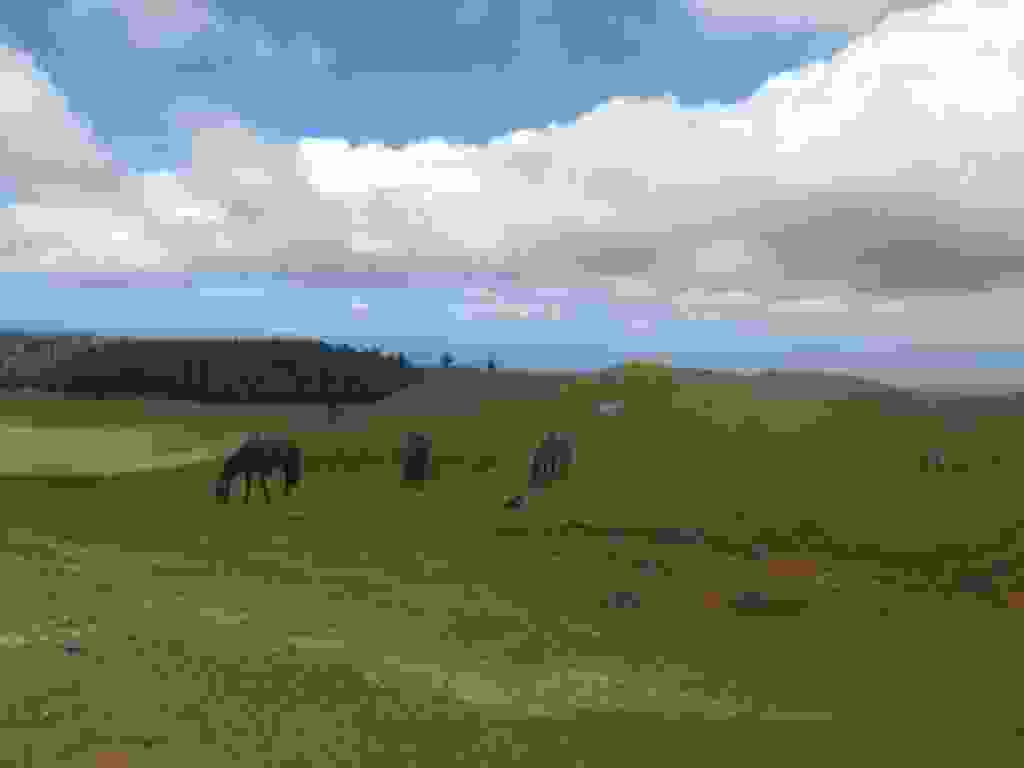
\includegraphics[width=\mywidth]{../wp-content/uploads/2015/03/P3022514-1024x768.jpg} \end{center}
\vspace{-\topsep}

\pagebreak
 Sandro et Carsten avec qui j'ai partagé la voiture. Sandro voyage depuis 8 ans sans interruption, record à battre !
\begin{center} 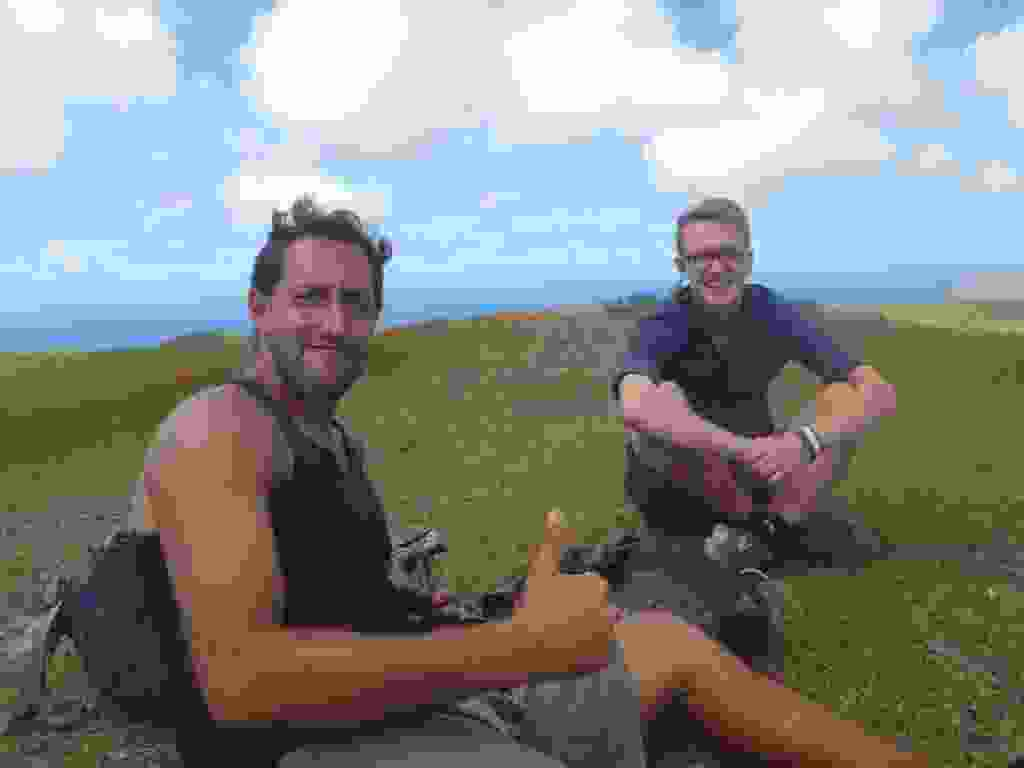
\includegraphics[width=\mywidth]{../wp-content/uploads/2015/03/P3022516-1024x768.jpg} \end{center}

Petit tour à la plage Anakena.\\
\begin{center} 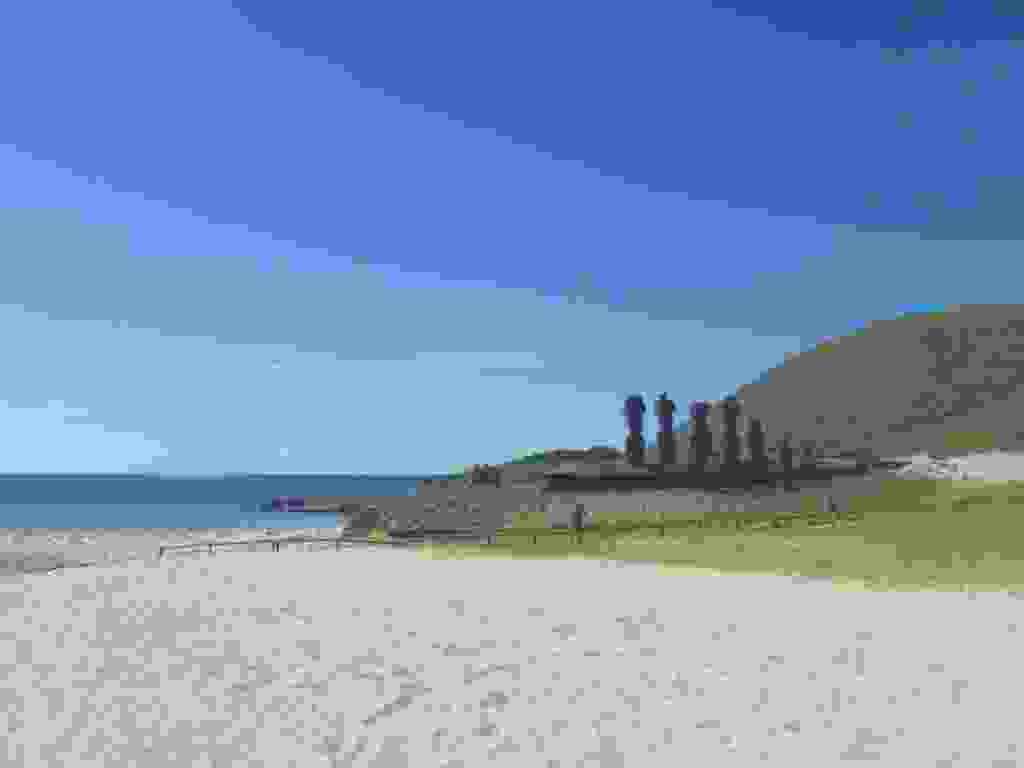
\includegraphics[width=\mywidth]{../wp-content/uploads/2015/03/P3032518-1024x768.jpg} \end{center}
\begin{center} 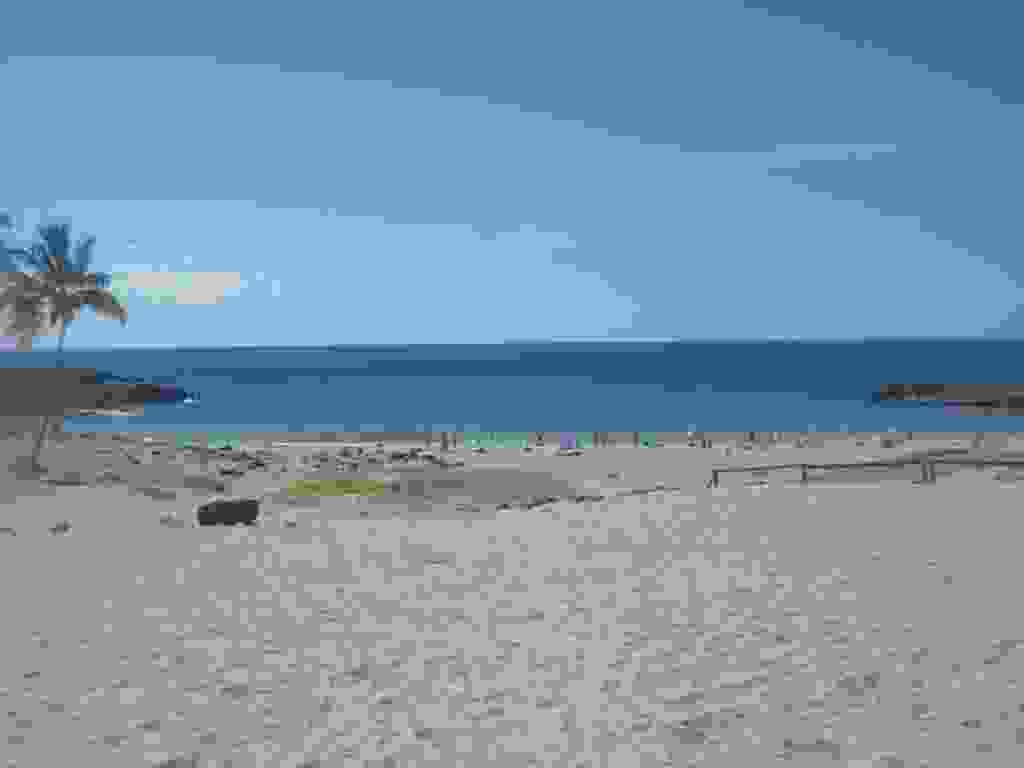
\includegraphics[width=\mywidth]{../wp-content/uploads/2015/03/P3032519-1024x768.jpg} \end{center}

Retour au village pour le coucher du soleil.
\begin{center} 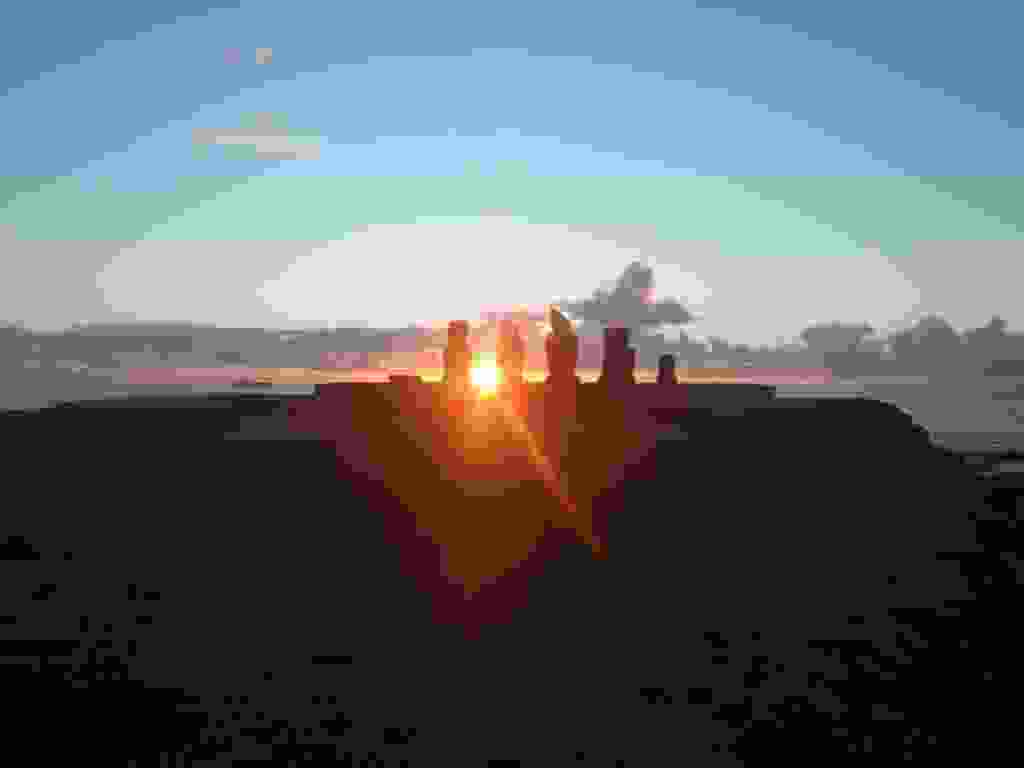
\includegraphics[width=\mywidth]{../wp-content/uploads/2015/03/P3032537-1024x768.jpg} \end{center}
\begin{center} 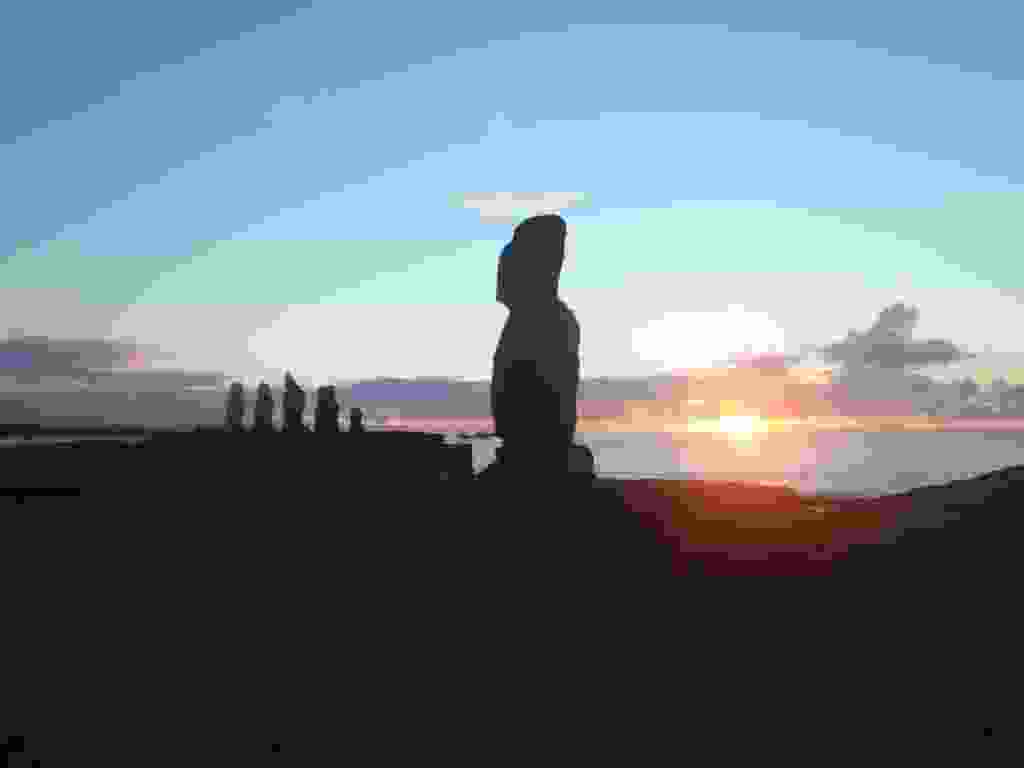
\includegraphics[width=\mywidth]{../wp-content/uploads/2015/03/P3032539-1024x768.jpg} \end{center}

 Petite rando le long de la côte, il y a quelques grottes à visiter dont une avec vue sur la mer !
\begin{center} 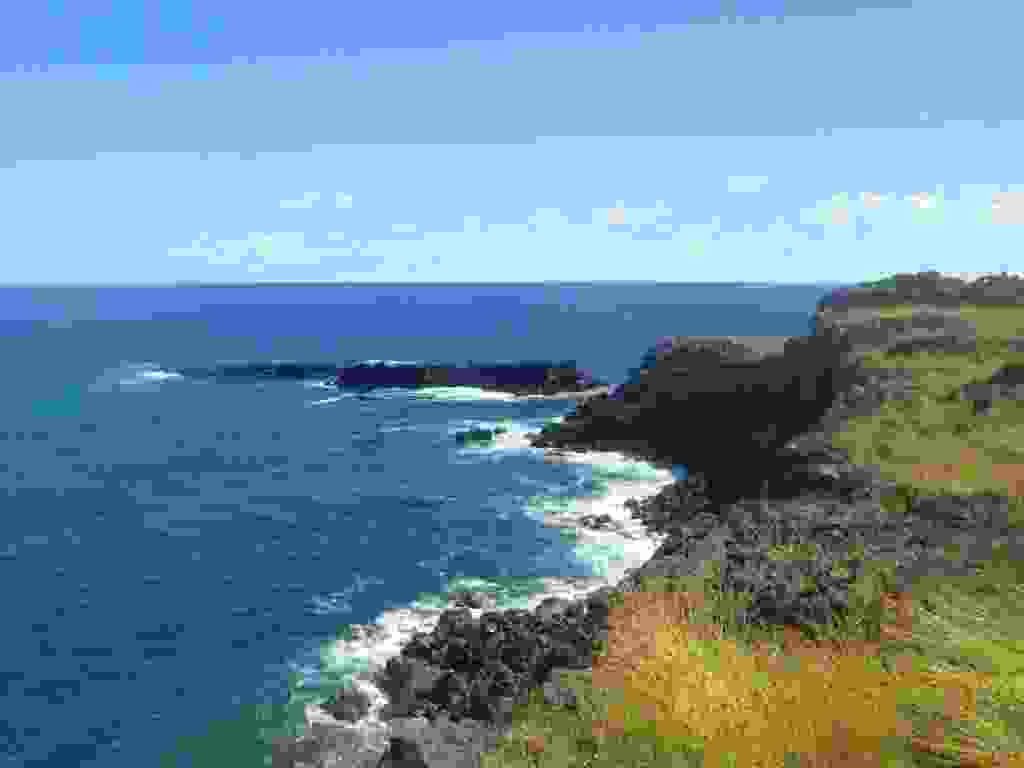
\includegraphics[width=\mywidth]{../wp-content/uploads/2015/03/P3032542-1024x768.jpg} \end{center}
\begin{center} 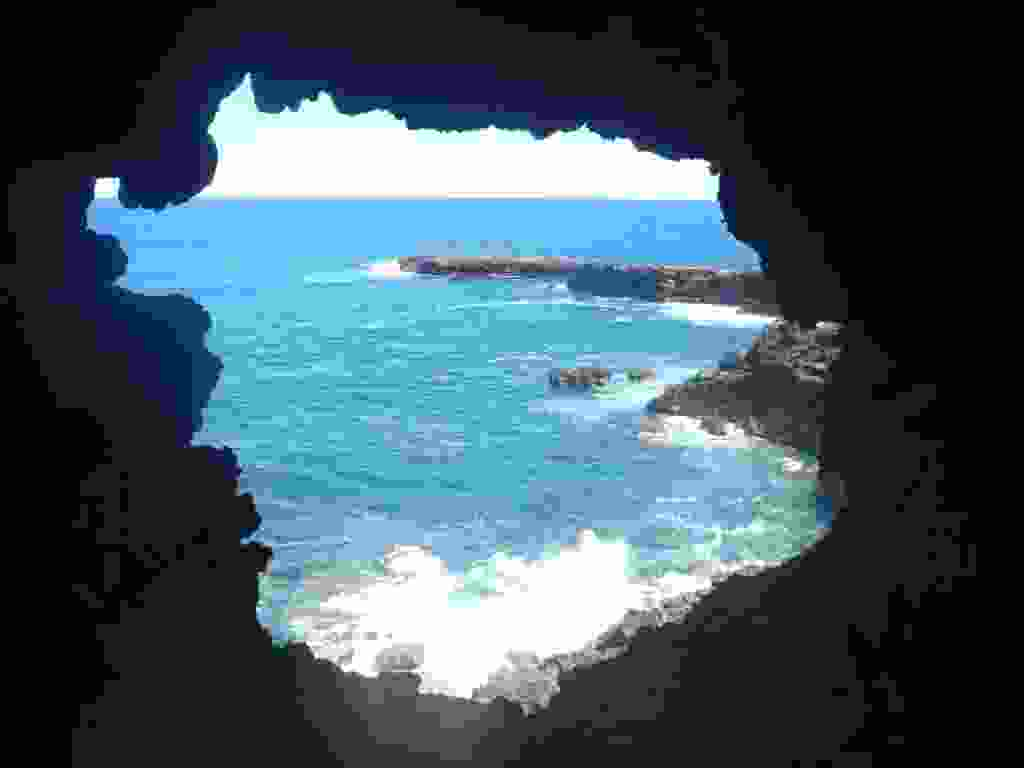
\includegraphics[width=\mywidth]{../wp-content/uploads/2015/03/P3032543-1024x768.jpg} \end{center}

 Site d'Orongo, lieu de cérémonie perché entre un cratère et l'océan Pacifique.
\begin{center} 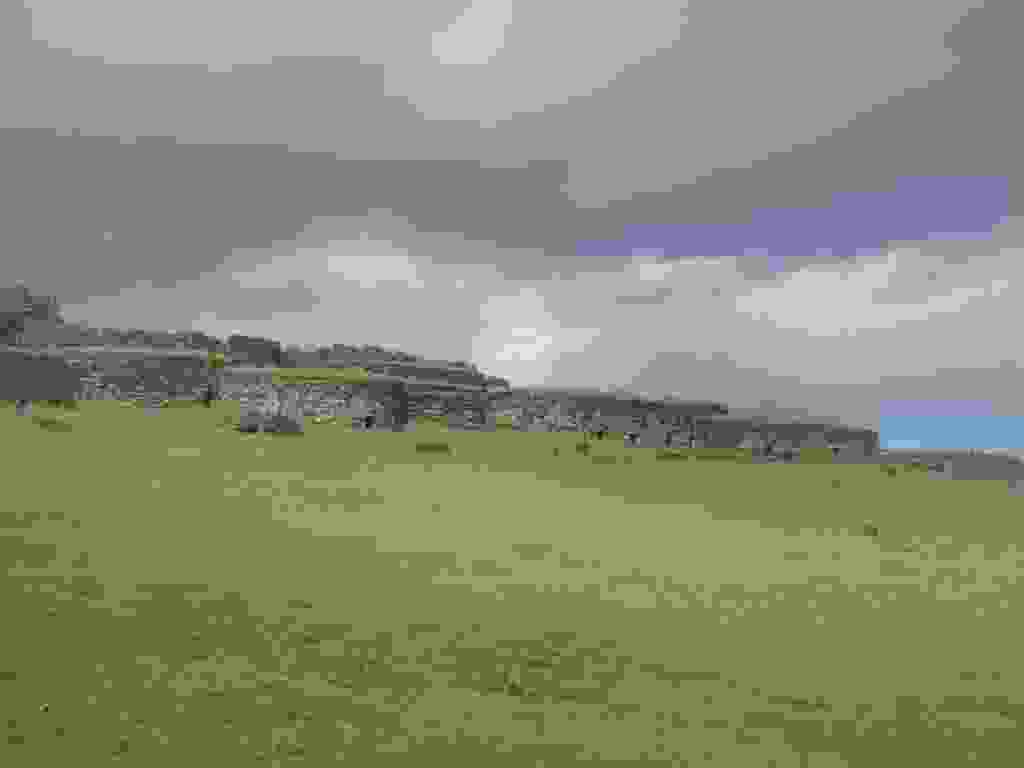
\includegraphics[width=\mywidth]{../wp-content/uploads/2015/03/P3042551-1024x768.jpg} \end{center}
\begin{center} 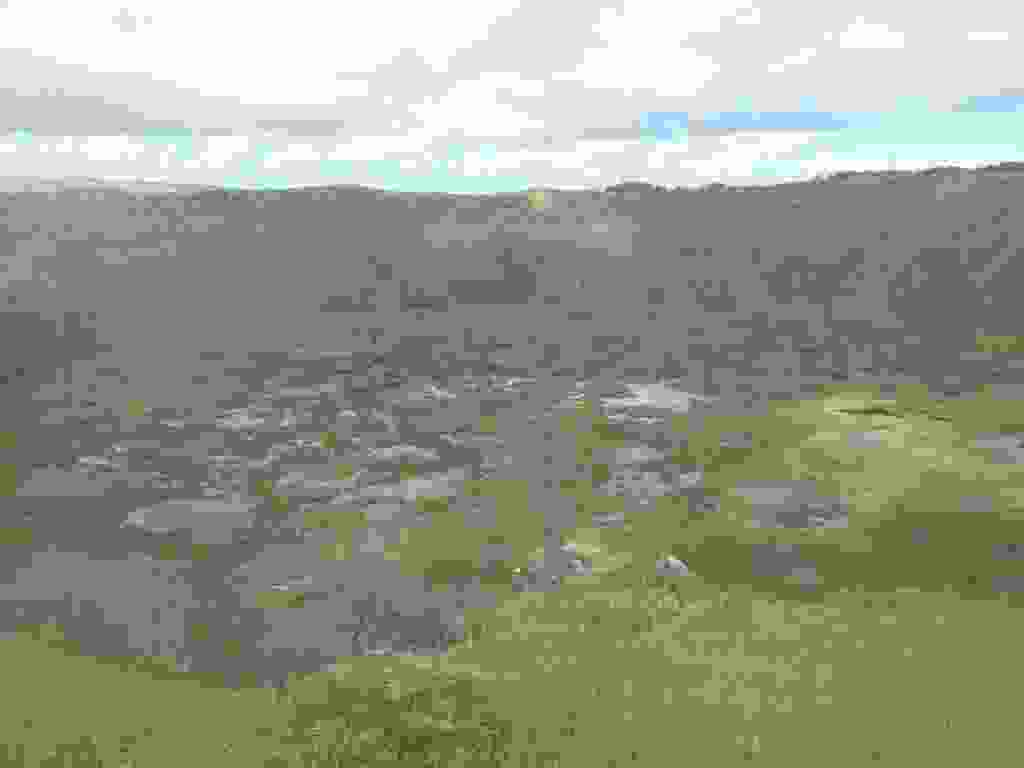
\includegraphics[width=\mywidth]{../wp-content/uploads/2015/03/P3042552-1024x768.jpg} \end{center}
\begin{center} 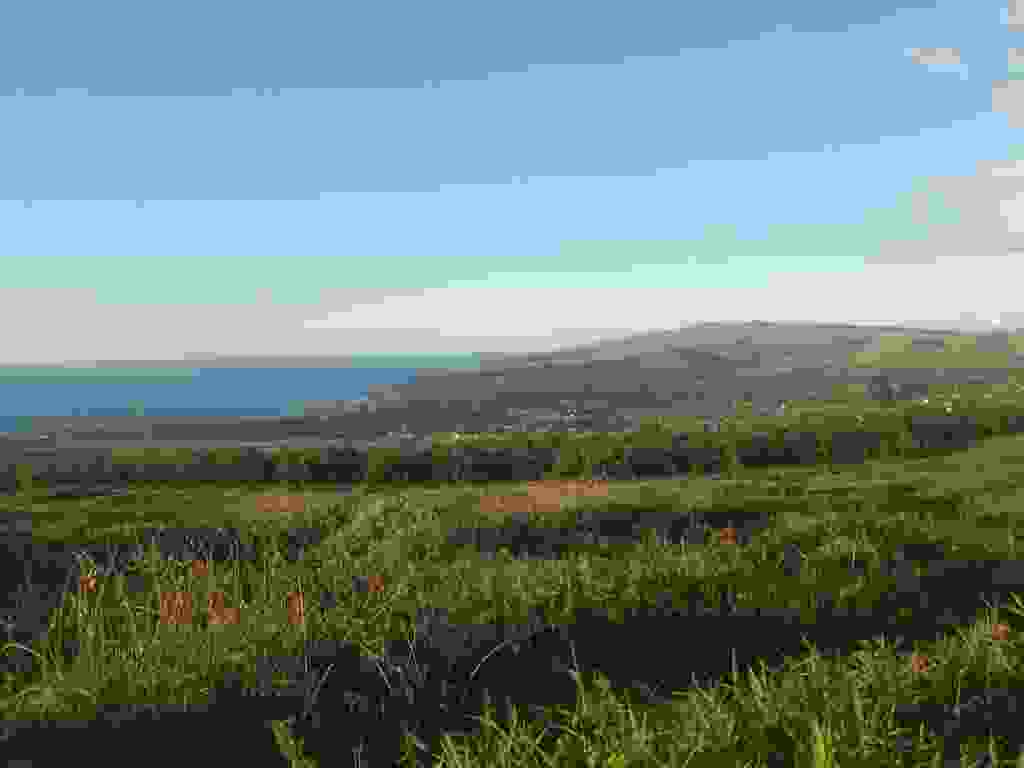
\includegraphics[width=\mywidth]{../wp-content/uploads/2015/03/P3032530-1024x768.jpg} \end{center}
\begin{center} 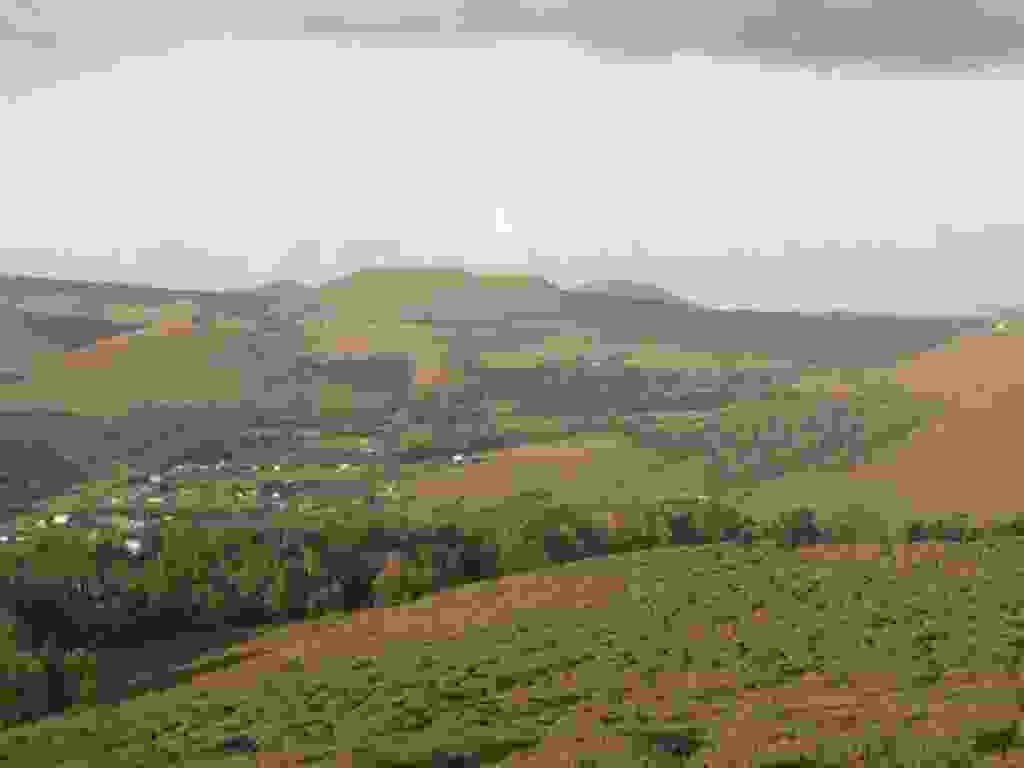
\includegraphics[width=\mywidth]{../wp-content/uploads/2015/03/P3032531-1024x768.jpg} \end{center}
